%% main.tex -- AAAI workshop draft.
%% Build with `make` (see README.md). Sections live in sections/, every measured
%% number lives in numbers.tex, and the one figure lives in figures/.
%%
%% Formatting follows the AAAI author kit. The kit's style file is not shipped
%% with this repository. When it is present, it is used exactly as the kit's own
%% template uses it. When it is absent, an approximate two-column layout is used
%% so the draft still compiles; that layout is NOT submittable, and the log says so.
\def\aaaistyle{aaai2026}% switch to the AAAI-27 kit's name once it is installed

\documentclass[letterpaper]{article}

\IfFileExists{\aaaistyle.sty}{%
  \usepackage[submission]{\aaaistyle}%
  \pdfinfo{/TemplateVersion (2026.1)}%
  \newcommand{\usingaaaikit}{}%
}{%
  \PackageWarningNoLine{main}{\aaaistyle.sty not found. Using an approximate
    layout that is not submittable. Install the AAAI author kit (README.md)}%
  \usepackage[letterpaper,top=0.75in,bottom=1.25in,hmargin=0.75in,
              columnsep=0.33in]{geometry}%
  \csname @twocolumntrue\endcsname% \makeatletter has no effect inside an argument
  \newcommand{\affiliations}[1]{}%
  \bibliographystyle{plainnat}%
}

% The AAAI kit's required packages and settings, in the kit's order.
\usepackage{times}
\ifdefined\nopsfonts % set by the Makefile when Helvetica/Courier metrics are absent
  \PackageWarningNoLine{main}{Helvetica and Courier metrics are not installed, so
    sans and mono fall back to Computer Modern. Output is not submittable
    (tlmgr install helvetic courier)}
  \renewcommand{\sfdefault}{cmss}% times.sty points these at phv and pcr
  \renewcommand{\ttdefault}{cmtt}%
\else
  \usepackage{helvet}
  \usepackage{courier}
\fi
\usepackage[hyphens]{url}
\usepackage{graphicx}
\urlstyle{rm}
\def\UrlFont{\rm}
\usepackage{natbib}
\usepackage{caption}
\frenchspacing
\setlength{\pdfpagewidth}{8.5in}
\setlength{\pdfpageheight}{11in}

% Additional packages. None is on the AAAI list of disallowed packages.
\usepackage{amsmath}
\usepackage{amssymb}
\usepackage{amsthm}
\usepackage{booktabs}
\usepackage{xspace}
\usepackage{tikz}
\usetikzlibrary{arrows.meta,calc}

% Sections are numbered so that cross-references resolve (the kit permits 1 or 2).
\setcounter{secnumdepth}{2}

\newtheorem{proposition}{Proposition}
\theoremstyle{remark}
\newtheorem*{remark}{Remark}

% Notation used throughout.
\newcommand{\R}{\mathbb{R}}
\newcommand{\softmax}{\operatorname{softmax}}
\newcommand{\LN}{\operatorname{LN}}
\newcommand{\eps}{\varepsilon}
\newcommand{\allclose}{\texttt{allclose}\xspace}
\newcommand{\arm}[1]{\textsc{#1}\xspace}
\newcommand{\RefArm}{\arm{reference}}
\newcommand{\DeclArm}{\arm{declarative}}
\newcommand{\HybArm}{\arm{hybrid}}

% Draft notes. Set \draftfalse to check that none remain before submitting.
\newif\ifdraft\drafttrue
\newcommand{\note}[1]{\ifdraft\textcolor{red}{[#1]}\fi}

%% numbers.tex -- every measured number the paper quotes, defined once.
%%
%% Rule: prose never types a measured number directly. It uses a macro from this
%% file, and each macro names the record it came from (paths are relative to the
%% repository root). Re-measuring something means editing one line here, and a
%% reviewer can audit every claim by reading this file next to docs/measurements/.
%% Tables are the one exception: a table's cells are literal, and the comment
%% directly above the table names the record they came from.
%%
%% Tags:  [M] measured and recorded in docs/measurements/
%%        [P] probe: reproduced by a script, not yet recorded in docs/measurements/
%%            (record it before submission; see README.md)

% ---------------------------------------------------------------------------
% Setup
% ---------------------------------------------------------------------------
% [M] docs/measurements/2026-08-17-first-hardware-run.md (header)
\newcommand{\gpuName}{NVIDIA A10}
\newcommand{\gpuArch}{sm\_86}
\newcommand{\tritonVersion}{3.3.0}
\newcommand{\torchVersion}{2.7.0}
% [M] src/autokernel_pbt/props/tasks.py (_LADDER_SHAPES); 9 shapes, two single-column
\newcommand{\ladderGroups}{9}
\newcommand{\ladderCeiling}{7/9}
% [M] src/autokernel_pbt/props/tolerance.py (DEFAULT_THRESH)
\newcommand{\refThresh}{30}
% [M] src/autokernel_pbt/props/oracle.py (AllcloseOracle defaults)
\newcommand{\allcloseRtol}{10^{-5}}
\newcommand{\allcloseAtol}{10^{-8}}
% [M] docs/measurements/2026-08-16-allclose-layernorm-false-positives.md
\newcommand{\atolBelowEps}{12}          % atol is ~12x below float32 eps

% ---------------------------------------------------------------------------
% Calibration: false positives on correct kernels
% ---------------------------------------------------------------------------
% [M] docs/measurements/2026-08-19-false-positive-rate.md
\newcommand{\fpGroups}{54}              % 6 correct kernels x 9 groups
\newcommand{\fpKernels}{6}
\newcommand{\fpAllclose}{10/54}
\newcommand{\fpAllcloseRate}{0.185}
\newcommand{\fpAllcloseLN}{5/9}
\newcommand{\fpAllcloseLNRate}{0.556}
% [M] docs/measurements/2026-08-18-autoresearch-loop-pbt-gate.md, section 4
\newcommand{\lnBrokenAllclose}{7/9}     % allclose on a *broken* layernorm
% [M] docs/measurements/2026-08-19-false-positive-rate.md, section 3
\newcommand{\sumsqWorstRatio}{48.1}     % layernorm_sumsq, shifted partner, (3,7)

% ---------------------------------------------------------------------------
% Reference-arm normalization
% ---------------------------------------------------------------------------
% [M] docs/superpowers/specs/2026-08-14-kernel-property-oracle-layer-design.md, 5.3
\newcommand{\linearNDrift}{127}         % correct-kernel ratio drift, n=64..16384
\newcommand{\linearNBlinder}{1500}      % detection floor vs allclose at n=4096
\newcommand{\logHeadroomLo}{213}
\newcommand{\logHeadroomHi}{779}
% [M] docs/measurements/2026-08-17-hybrid-reduction-tree.md
\newcommand{\multiTileLogDrift}{5.9}
\newcommand{\multiTileOneDrift}{7.6}
\newcommand{\multiTileTileAwareDrift}{3.5}
\newcommand{\multiTileMaxTiles}{256}

% ---------------------------------------------------------------------------
% Detection: mutation corpora
% ---------------------------------------------------------------------------
% [M] docs/measurements/2026-08-17-provisional-corpus-pilot.md
% [M] docs/measurements/2026-08-17-blinded-corpus-pilot.md
% [M] docs/measurements/2026-08-18-arm-differentiation-null-result.md
\newcommand{\mutantsAdmitted}{20}
\newcommand{\armDisagreements}{0}
\newcommand{\contamRejection}{0.00}
\newcommand{\blindRejection}{0.20}
\newcommand{\grownRejectionLadder}{0.27}
\newcommand{\grownRejectionScale}{0.73}
\newcommand{\grownTolFree}{3/11}
% [M] reference/PBT-property-based-testing/README.md (ISSTA 2026 taxonomy)
\newcommand{\isstaBugs}{301}
\newcommand{\isstaSpecialization}{80}
\newcommand{\isstaDtype}{58}
% [M] docs/measurements/2026-08-17-blinded-corpus-pilot.md (widest ladder row)
\newcommand{\ladderWidestRow}{129}

% ---------------------------------------------------------------------------
% Cross-backend transfer and scale
% ---------------------------------------------------------------------------
% [M] docs/measurements/2026-08-17-first-hardware-run.md
\newcommand{\firstRunRows}{52}
% [M] docs/measurements/2026-08-17-at-scale-hardware-run.md
\newcommand{\scaleElements}{29.4\,M}
\newcommand{\scaleRoofline}{78}         % percent of A10 peak bandwidth
\newcommand{\tileTailRowSum}{1.51}      % BLOCK=2048 at n=4096: rows sum to 1.5089

% ---------------------------------------------------------------------------
% The autoresearch loop
% ---------------------------------------------------------------------------
% [M] docs/measurements/2026-08-18-autoresearch-loop-pbt-gate.md, section 1
\newcommand{\loopCandidates}{26}
\newcommand{\loopRounds}{6}
\newcommand{\loopRejections}{0}
\newcommand{\loopBpbBase}{2.829}        % 2.8287, sd 0.0104, 3 seeds
\newcommand{\loopBpbBest}{2.228}        % 2.2280, sd 0.0147, 3 seeds
\newcommand{\loopBpbGain}{21.2}         % percent
\newcommand{\loopTputBase}{40.1}        % k tok/s (40072)
\newcommand{\loopTputBest}{51.2}        % k tok/s (51166)
\newcommand{\loopTputGain}{27.7}        % percent
\newcommand{\loopGateLines}{140}
% [M] same record, section 3 (author-chosen saboteurs; three were timed)
\newcommand{\sabCount}{6}
\newcommand{\sabSpeedNoMax}{1.11}
\newcommand{\sabSpeedNoCenter}{1.76}
\newcommand{\sabSpeedNoDivide}{2.40}
% [M] same record, section 5
\newcommand{\fastExpRelErr}{4.5\times10^{-6}}
\newcommand{\fastExpWorse}{40}
% [M] same record, section 7
\newcommand{\wdCoverage}{7.7}           % percent of parameters weight decay reached

% ---------------------------------------------------------------------------
% Incompleteness of the property bundles
% ---------------------------------------------------------------------------
% [M] docs/measurements/2026-10-01-softmax-temperature-blind-spot.md
\newcommand{\betaSweepValues}{16}
\newcommand{\betaFirstCatch}{16}
\newcommand{\refRatioLo}{1.1\times10^{6}}
\newcommand{\refRatioHi}{4.0\times10^{6}}
\newcommand{\spreadExact}{4.8}
\newcommand{\spreadFastExp}{48}
\newcommand{\spreadBetaTwo}{5.2\times10^{7}}
\newcommand{\spreadBetaNeg}{1.04\times10^{8}}
\newcommand{\spreadControl}{4.3}
\newcommand{\bpbCorrect}{2.2292}
\newcommand{\bpbBetaTwo}{2.2279}
\newcommand{\bpbFill}{3.790}
\newcommand{\fillSpeedup}{52--54}
% [P] symmetry probe, re-run 2026-10-01 against pbt_gate.check_task, unmodified,
%     GATE_SEED=42, NumPy 1.26.4. Script: symmetry_probe.py (not yet in the repo).
\newcommand{\probeFamilies}{6}
\newcommand{\gapFamiliesTotal}{10}      % 4 temperature rows + 6 probe rows

% ---------------------------------------------------------------------------
% Methodology findings in our own instrument
% ---------------------------------------------------------------------------
% [M] design spec 5.3 (shift relation scaled to the failure mechanism)
\newcommand{\shiftUnitCatch}{0}         % percent, 400 trials
\newcommand{\shiftScaledCatchLo}{11.8}
\newcommand{\shiftScaledCatchHi}{18.0}
% [M] design spec 6.5 (REPLAY_FAIRNESS passed vacuously through three fixes)
\newcommand{\fairnessLayers}{3}
\newcommand{\relabelLoss}{14/14}
% [M] CLAUDE.md (review standard; module-contract table on branch widen-corpus-coverage)
\newcommand{\reviewDefects}{20}
\newcommand{\contractCount}{22}
% [M] docs/measurements/2026-08-17-sanitizer-viability-probe.md
\newcommand{\sanitizerOverrun}{1\,MB}

% ---------------------------------------------------------------------------
% The formal track (feature 0009 built; 0010 and 0011 planned)
% ---------------------------------------------------------------------------
% [M] branch formal-adherence (commits 82d47d8..9ed8ca9, not yet merged):
%     specs/features/0009-formal-core/, src/autokernel_pbt/formal/,
%     tests/unit/formal/. Suite: 641 passed, 1 skipped.
\newcommand{\formalChecks}{6}
\newcommand{\formalRemovedConditions}{20}   % conditions deleted one at a time, each caught
% [M] docs/superpowers/specs/2026-10-01-agent-formal-adherence-design.md (on that branch)
\newcommand{\pilotLanguages}{7}
\newcommand{\pilotTargets}{7}
\newcommand{\pilotReplicates}{3}
\newcommand{\pilotSessions}{147}
\newcommand{\axiomSamples}{4096}

% ---------------------------------------------------------------------------
% Proofs about the oracle (Proposition 1 mechanized)
% ---------------------------------------------------------------------------
% [M] docs/measurements/2026-10-01-softmax-bundle-mechanized.md; proofs/softmax-bundle/
\newcommand{\leanTheorems}{6}
\newcommand{\leanLines}{367}
\newcommand{\leanVersion}{4.33.0}
\newcommand{\expAxioms}{3}            % positive, additive, injective

% ---------------------------------------------------------------------------
% External numbers (cited, not ours)
% ---------------------------------------------------------------------------
% costa2026aicompiler, best provable vs best tested GEMM speedup
\newcommand{\provableGemm}{0.24}
\newcommand{\testedGemm}{1.03}


\title{Skills, Properties, Proofs:\\
       A Harness for Long-Running Kernel-Optimizing Agents}
\author{Anonymous Submission}
\date{}
\affiliations{}

\begin{document}

\maketitle

\begin{abstract}
An agent that optimizes compute kernels faces an objective whose two halves pull
apart: many of the cheapest ways to make a kernel faster also make it wrong. The
incorrect ``optimizations'' we timed run up to \sabSpeedNoDivide$\times$ faster
than the correct kernel, and a constant-fill ``softmax'' runs \fillSpeedup$\times$
faster \emph{and passes our own property gate}. The correctness gate is therefore
half of the fitness function, and its calibration and completeness bound what a
long-running agent can reach. We describe a harness with three layers: agent
\emph{skills} that carry measured lessons across sessions and control what each
sub-agent may see; \emph{property-based testing} over byte-identical replayed
executions, which serves as a cheap and calibrated gate; and \emph{formal proof},
which certifies that the gate's laws pin down the specification. Comparing four oracle
strategies on NumPy and Triton (\gpuName), we find that they never disagree on
\mutantsAdmitted{} mutants from three corpora; that the field-default \allclose
rejects \fpAllcloseRate{} of correct-kernel groups while the others reject none,
so an \allclose-gated loop cannot accept its own baseline; and that a
property-gated loop improves validation bits-per-byte by \loopBpbGain\% at
\loopTputGain\% higher throughput. We also show that the property bundles are
incomplete: they admit \gapFamiliesTotal{} wrong kernels, which we characterize
exactly and close with one law per task. Last, we describe the formal layer. An
agent writes the spec, a model of the kernel and the proof in each of seven formal
languages, and six checks decide whether the proof certifies anything. Those checks
execute every formal artifact on the PBT cases and catch each kind of spec gaming.
Their core is built, and the pilot is pre-registered.
\end{abstract}

\section{Introduction}
\label{sec:intro}

Language-model agents now write and optimize GPU kernels in long, autonomous loops:
propose a change, check it, measure it, keep it or revert it
\citep{ouyang2025kernelbench,lange2025robust,karpathy2026autoresearch}. The check is
usually \allclose against a reference implementation, and the literature has begun
to document what slips past it: kernels that skip work, overfit the tested shapes or
read the reference's answer \citep{lange2025robust,sarkar2026illusion}.

The problem is structural, not incidental. In an autoresearch loop that trains a
model, the metric is held-out loss, so search pressure and correctness pressure point
the same way: a wrong model simply scores worse. In kernel optimization they point in
opposite directions. Dropping the max-subtraction from a softmax, or the centering
and the divide from a layernorm, makes the kernel \sabSpeedNoMax--\sabSpeedNoDivide$\times$
faster in our measurements, and each produces plausible output. The correctness gate
is not an auxiliary check bolted onto the loop. It is half of the fitness function, and
two of its properties decide what the loop can reach. \emph{Calibration}: does the gate
accept correct kernels that differ from the reference in the last bits, as every
optimized kernel does? \emph{Completeness}: does it reject every wrong kernel the agent
can cheaply find? A third property, the gate's cost, decides how many iterations the
loop can afford.

We built a harness around these three requirements, one layer each
(Figure~\ref{fig:harness}):
\begin{itemize}
  \item \textbf{Skills}: versioned, natural-language procedures loaded into an agent's
    context. They carry what earlier sessions measured, so that later agents neither
    rediscover it nor exploit it, and they set what each sub-agent is allowed to see.
  \item \textbf{Property-based testing (PBT)}: a gate built from algebraic laws and
    metamorphic relations, evaluated offline over byte-identical replayed executions, so
    that competing oracles can be compared fairly and the gate costs milliseconds.
  \item \textbf{Formal proof}: agent-written proofs that a kernel adheres to its
    specification, issued as certificates only after the gate accepts the kernel. The
    agent writes the spec too. Six checks, run on PBT's own executions, decide whether a
    proof certifies anything.
\end{itemize}

\paragraph{Contributions.}
\begin{enumerate}
  \item A controlled comparison of four oracle strategies (\allclose, a
    LAPACK-style normalized test ratio, a declarative property bundle and a hybrid)
    over identical recorded executions on NumPy and Triton (\S\ref{sec:calibration},
    \S\ref{sec:detection}). The four tie on detection. They differ sharply on false
    positives, and the field default cannot gate a loop at all.
  \item A property-gated autoresearch loop and a saboteur matrix showing that the gate
    has teeth and that the reachable frontier depends on the choice of oracle
    (\S\ref{sec:loop}).
  \item An exact characterization of the property bundles' solution sets, showing ten
    admitted wrong kernels, including one \fillSpeedup$\times$ faster than the real
    kernel, and a one-law completion for each task (Proposition~\ref{prop:softmax},
    \S\ref{sec:incomplete}).
  \item Evidence that skills shape what agents produce: blinding the mutant authors changed
    the corpus, and naming reward hacks in the loop's instructions changed what agents
    proposed (\S\ref{sec:skills-results}).
  \item A certificate design for agent-written proofs, in which the agent writes the spec
    as well and spec gaming is measured rather than forbidden. Each of its six checks is
    the sole catcher of one cheat. The checks' core is built, and a seven-language pilot is
    pre-registered (\S\ref{sec:formal}, \S\ref{sec:program}).
\end{enumerate}

The skills and PBT layers are built and measured. Of the formal layer, the
language-neutral checking core is built, and the first proof about the oracle, Proposition~\ref{prop:softmax}(a,b),
is machine-checked. No agent has written a proof yet. We
label every claim as measured, built or planned.

\section{Related Work}
\label{sec:related}

\paragraph{Checking LLM-generated kernels.}
KernelBench scores generated kernels by \allclose against a PyTorch reference
\citep{ouyang2025kernelbench}. Several 2025--26 studies show this oracle is inadequate.
Agents exploit benchmark loopholes \citep{lange2025robust}, kernels that pass are often
wrong \citep{sarkar2026illusion}, and boundary-shape input generation finds more bugs
than adversarial values at far lower false-positive cost \citep{sarkar2026inputs}.
Declarative kernel contracts \citep{veit2026contracts,shah2026contract} and
tensor-algebraic property skeletons for DL compilers \citep{qiu2026propilot} already
exist as concepts. A taxonomy of \isstaBugs{} real bugs in tile-based GPU programs
\citep{rathnasuriya2026tile} supplies the fault classes we use to author mutants. A
recent systematic review observes that LLM test oracles are mostly judged by how closely
they resemble a known oracle, not by the faults they catch \citep{mughal2026oracles}. Our
comparison scores oracles by the faults they catch, with the test budget held fixed by
construction. Mutation analysis supports exactly this ordinal use
\citep{andrews2005mutation,just2014mutants,papadakis2018mutation}.

\paragraph{Property-based and metamorphic testing.}
PBT \citep{claessen2000quickcheck,maciver2019hypothesis} and metamorphic testing
\citep{chen2018metamorphic,barr2015oracle} replace example outputs with laws and
relations. \citet{hughes2020specify} found that model-based properties, the analogue of our
reference arm, caught every planted bug about ten times faster than metamorphic ones. He
argued that metamorphic properties earn their place where the model is expensive or
would repeat the implementation's bugs. Our detection results reproduce his finding for
kernels that have a cheap trusted reference. LLMs can draft such properties
\citep{vikram2023pbt}. We treat drafted bundles as artifacts whose completeness must be
established rather than assumed. For numerical tolerances we follow LAPACK's normalized
test ratios \citep{anderson1992lawn41} and the rounding-error analysis of
\citet{higham2002accuracy} and \citet{higham2019probabilistic}.

\paragraph{Formal methods for kernels and verifier-guided agents.}
VOLTA checks equivalence of GPU kernels soundly and completely for a statically
analyzable class, treating floats as reals \citep{dubey2025volta}. VeriTile reasons about
Triton-style kernels in Lean~4 \citep{veritile2026,demoura2021lean4}. ATL proves scheduling
rewrites of tensor programs correct in Coq \citep{liu2022atl}. Making proof a hard gate
on kernel code is costly: when an agent lowers Triton kernels to PTX, the best provable
GEMM ran at \provableGemm$\times$ against \testedGemm$\times$ for the best tested one
\citep{costa2026aicompiler}. Agents now write verified code against given specs in Dafny,
Verus and Lean \citep{loughridge2024dafnybench,bursuc2025vericoding}, and agent-written
specs have been scored against held-out ground truth
\citep{ye2025verina,thakur2025clever}. Verifier feedback improves those attempts
\citep{aggarwal2025alphaverus}. None of this work targets numerical GPU kernels or
floating point, or profiles how agents game their own specs. Industrial practice pairs a
proven model with differential random testing of the production code
\citep{disselkoen2024cedar}. We take the same division of labour: proofs about the oracle
and the plan, tests on the code.

\paragraph{Agent skills and long-running loops.}
Agent skills package procedural knowledge as files an agent loads on demand
\citep{anthropic2025skills}. autoresearch runs a fixed-budget keep-or-revert loop guided
by a natural-language program \citep{karpathy2026autoresearch}. We use skills in both
roles, as memory between sessions and as the specification of what an experiment's
sub-agents may see.

\section{The Harness}
\label{sec:harness}

%% figures/harness.tex -- Figure 1, the harness. Solid boxes are built and
%% measured. Dashed ones belong to the formal track, whose checking core is built
%% but which no formal language or agent has run yet.
\begin{figure}[t]
\centering
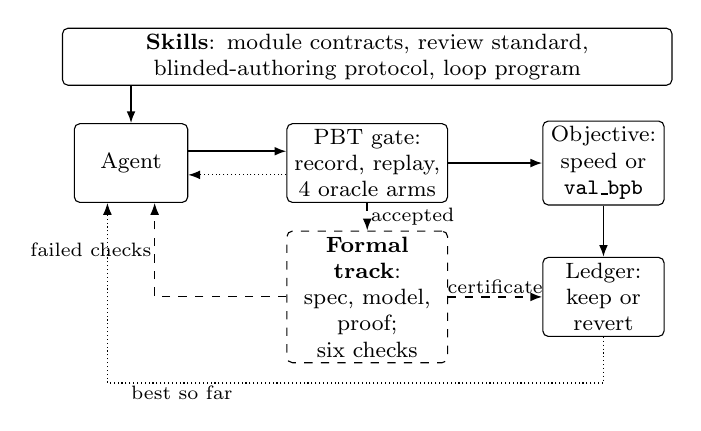
\begin{tikzpicture}[
    font=\footnotesize,
    box/.style={draw, rounded corners=2pt, align=center, inner sep=2pt,
                minimum height=10mm},
    planned/.style={box, dashed},
    flow/.style={-{Latex[length=1.5mm]}, semithick},
    back/.style={-{Latex[length=1.5mm]}, densely dotted},
    lbl/.style={font=\scriptsize, inner sep=1pt},
  ]
  \node[box, text width=13mm] (agent) at (0,0) {Agent};
  \node[box, text width=19mm] (gate) at (3.0,0) {PBT gate:\\record, replay,\\4 oracle arms};
  \node[box, text width=14mm] (obj) at (6.0,0) {Objective:\\speed or\\\texttt{val\_bpb}};
  \node[box, text width=76mm, minimum height=7mm] (skills) at (3.0,1.35)
    {\textbf{Skills}: module contracts, review standard, blinded-authoring
     protocol, loop program};
  \node[planned, text width=19mm] (formal) at (3.0,-1.7)
    {\textbf{Formal track}:\\spec, model, proof;\\six checks};
  \node[box, text width=14mm] (ledger) at (6.0,-1.7) {Ledger:\\keep or\\revert};
  \coordinate (bottom) at ($(formal.south) + (0,-2.5mm)$);

  % main flow
  \draw[flow] ([yshift=1.5mm]agent.east) -- ([yshift=1.5mm]gate.west);
  \draw[flow] (gate) -- (obj);
  \draw[flow] (obj) -- (ledger);
  \draw[flow] (skills.south -| agent.north) -- (agent.north);
  \draw[flow, dashed] (gate) -- node[lbl, right] {accepted} (formal);
  \draw[flow, dashed] (formal) -- node[lbl, above] {certificate} (ledger);
  % feedback to the agent
  \draw[back] ([yshift=-1.5mm]gate.west) -- ([yshift=-1.5mm]agent.east);
  \draw[back] (ledger.south) -- (ledger.south |- bottom)
    -- node[lbl, below, pos=0.85] {best so far} ([xshift=-3mm]agent.south |- bottom)
    -- ([xshift=-3mm]agent.south);
  \draw[back, dashed] (formal.west) -| node[lbl, left, pos=0.75] {failed checks}
    ([xshift=3mm]agent.south);
\end{tikzpicture}
\caption{The harness. An agent proposes a candidate with its skills in context. The
  PBT gate scores it on recorded executions, and admitted candidates are measured on the
  objective and kept or reverted. Dotted arrows are feedback to the agent:
  counterexamples from the gate, and the best candidate so far. The formal track
  (dashed) issues certificates only for kernels the gate accepted. The agent writes
  the spec, the model and the proof, and six checks run on PBT's executions decide
  whether the proof counts. Its checking core is built, but no language has run yet.}
\label{fig:harness}
\end{figure}


Figure~\ref{fig:harness} shows one iteration. An agent edits a candidate kernel, the
PBT gate scores it, and only admitted candidates are measured on the loop's objective.
That objective is kernel speed in a kernel-optimization loop, or validation
bits-per-byte (\texttt{val\_bpb}) when the kernels sit inside a model being trained.
A ledger keeps or reverts the candidate. The three layers below divide the work.

\subsection{Skills}
\label{sec:skills}

A skill is a versioned document that an agent loads into its context: a procedure, a
set of rules, or a record of what not to rediscover \citep{anthropic2025skills}. Long
sessions and fresh sub-agents lose what earlier ones measured unless it is written
down where the next agent will read it. Four skills carry the weight in this work.
\begin{itemize}
  \item \textbf{Module contracts.} The repository's agent notes record more than
    \contractCount{} contracts, each of which once cost a review round to establish. For
    example: a reduction's tolerance takes the reduction length explicitly; PyTorch's
    caching allocator hides out-of-bounds accesses from \texttt{compute-sanitizer}; and a
    Triton tile narrower than its row silently drops the row's tail.
  \item \textbf{The review standard.} Every assertion in a test must be the
    \emph{unique} catcher of at least one deliberately broken implementation (a
    saboteur). This is verified by deleting each assertion in turn and checking that
    exactly its own saboteurs survive.
  \item \textbf{The blinded-authoring protocol.} An agent writing a mutant receives the
    correct kernel and one verbatim fault-class description from the bug taxonomy
    \citep{rathnasuriya2026tile}, and nothing else. It never sees the property set,
    tolerances, other mutants or results. Here the skill specifies what is
    \emph{withheld}.
  \item \textbf{The loop program.} The instructions for the optimizing agent name the two
    cheapest reward hacks and their measured speedups, state each kernel's semantics, and
    point to the measured headroom.
\end{itemize}

\subsection{Property-based testing over replayed executions}
\label{sec:pbt}

\paragraph{Record, then replay.}
A seeded generator emits \emph{case groups}: a base input plus metamorphic partners
that share a group identity, such as $x$ and $x + c\mathbf{1}^\top$ with one constant
per row. The whole batch executes once on one backend, and inputs, outputs and device
telemetry are persisted (tensors to safetensors, rows to Parquet). Every oracle is then
evaluated \emph{offline} over the same bytes. This makes the comparison fair by
construction, since no oracle influences which inputs another sees, and a recorded hardware run
can be re-scored by a new oracle without touching a device. Oracles return
\textsc{pass}, \textsc{fail} or \textsc{inconclusive}, so that a case where no
judgment is defined is never counted as a caught bug. The unit of every rate is the
case group.

\paragraph{Four oracle arms.}
\allclose is the field default, \texttt{np.allclose} against the reference with
$\mathrm{rtol}=\allcloseRtol$ and $\mathrm{atol}=\allcloseAtol$. It is deliberately
untuned. \RefArm replaces elementwise comparison with a LAPACK-style normalized test ratio
\citep{anderson1992lawn41}:
\begin{equation}
  r(\hat y, y) \;=\; \frac{\lVert \hat y - y \rVert_\infty}
       {\lVert y \rVert_\infty \cdot \eps_{\text{dtype}} \cdot \max(\log_2 n,\, 1)}
  \;\le\; \refThresh,
  \label{eq:ratio}
\end{equation}
where $n$ is the reduction length and $\log_2 n$ is the error bound for pairwise
summation \citep{higham2002accuracy}. \DeclArm evaluates a per-task bundle of laws and never
consults a reference. For softmax the bundle is: every output is finite, every output
lies in $[0,1]$, every row sums to one, and the output is invariant under per-row input
shifts. For layernorm it is: finite outputs, zero row mean, unit row variance and shift
invariance. Tolerances for the bundles come from each dtype's rounding budget. \HybArm
evaluates the laws first and recomputes the reference only when the laws find nothing.

\paragraph{Corpus and backends.}
Development uses a ladder of \ladderGroups{} shapes per task, from $(8,8)$ to $(7,129)$,
with the degenerate rungs $(1,1)$ and $(17,1)$. On single-column rows softmax is
identically $1$ for \emph{any} implementation, so \ladderCeiling{} is the most any arm
can detect on softmax, and every absolute rate below is deflated by that constant. Shift
partners are scaled to $\tfrac12\log(\text{float max})$, the regime where a missing
max-subtraction actually overflows. Kernels run on a NumPy backend and on Triton
\tritonVersion{} on an \gpuName{} (\gpuArch) behind one backend interface.

\subsection{Formal proof: agent-written certificates}
\label{sec:formal}

A test can only check the properties it was given. A formal statement can say that a
kernel computes a function. In our design the kernel-writing agent writes everything
in a formal language: a \emph{spec} formalizing the informal one, a \emph{model} of the
kernel, \emph{hypotheses} under which it claims adherence, and a \emph{proof} of a
theorem whose shape the harness fixes, $\forall x.\; H(x) \Rightarrow S(x, M(x))$. An
agent rewarded for an accepted proof has cheaper routes than proving adherence. It can
weaken the spec, model a simpler kernel, assume a hypothesis nothing satisfies, or
rely on a false axiom. The gate's blind spot (\S\ref{sec:incomplete}) is the first of
these, committed by a person. We therefore let the agent write the spec on purpose and
\emph{measure} the gaming.

%% Source: docs/superpowers/specs/2026-10-01-agent-formal-adherence-design.md, section 5.
\begin{table}[t]
\centering
\small
\setlength{\tabcolsep}{3pt}
\begin{tabular}{@{}lp{0.40\columnwidth}p{0.40\columnwidth}@{}}
\toprule
& Establishes & Sole-catcher cheat \\
\midrule
C1 & checker accepts the proof, no escape hatch & proof ends in \texttt{sorry} \\
C2 & spec accepts the reference's outputs & spec is the kernel, bit for bit \\
C3 & spec rejects every wrong output held, the kernel's own included & spec made of the gate's four laws \\
C4 & model matches the real kernel's executions & model of a tail-dropping kernel computes the whole row \\
C5 & hypotheses hold on every case & $\texttt{BLOCK} \ge n$ on a launch with $\texttt{BLOCK} < n$ \\
C6 & axioms hold on samples; no derivation of \textsf{False} & axiom $\exp(x) = 1 + x$ \\
\bottomrule
\end{tabular}
\caption{The six checks a proof must pass to certify adherence. Each is the only check
  that rejects its cheat. C2--C6 run each artifact's executable reading on PBT's
  cases, with comparisons and tolerances the harness owns.}
\label{tab:checks}
\end{table}

A proof certifies adherence only if all \formalChecks{} checks in Table~\ref{tab:checks}
pass. Every artifact must have an executable reading, obtained from the proved
definitions themselves (for example, a definition over an abstract numeric type
instantiated at IEEE floats). The PBT machinery then executes the formal claims on its
own cases, backends and rounding budget. The agent never sees those cases. C2 and C3
pin the spec between the reference and a hidden set of wrong kernels that includes
every row of Table~\ref{tab:gap}. A spec loose enough to admit the gate's failures fails
C3, and one too tight to accept the reference fails C2. Certificates are issued only for
kernels the gate has already accepted, and never act as the loop's filter, because a
proof gate costs speed \citep{costa2026aicompiler}.

\paragraph{Status.} The language-neutral core that runs C2--C6 is built and tested
against a fake language adapter. Each check rejects its own cheat and no other, and
deleting any of \formalRemovedConditions{} conditions inside the checks fails a test.
Its review found one way to certify a wrong kernel. The disjunctive spec
``$y = \softmax(x)$ or $y = \softmax(1.5x)$'' certified a $\softmax(1.5x)$ kernel,
because C3 probed only the hidden set. C3 now also probes the kernel under proof. No
formal language or agent has run yet (\S\ref{sec:program}).

\section{Results}
\label{sec:results}

All rates are fractions of case groups. Device runs used Triton \tritonVersion{} and
PyTorch \torchVersion{} on one \gpuName{}, with seed 42 and float32 throughout.

%% Source: docs/measurements/2026-08-19-false-positive-rate.md, section 1.
\begin{table}[t]
\centering
\small
\begin{tabular}{@{}llcc@{}}
\toprule
Correct kernel & Task & \allclose & Other three \\
\midrule
stock                       & softmax   & 0/9 & 0/9 \\
\texttt{exp2} rewrite       & softmax   & 0/9 & 0/9 \\
reciprocal-multiply         & softmax   & 0/9 & 0/9 \\
stock                       & relu      & 0/9 & 0/9 \\
stock                       & layernorm & \textbf{5/9} & 0/9 \\
\texttt{rsqrt} rewrite      & layernorm & \textbf{5/9} & 0/9 \\
\midrule
pooled                      &           & \textbf{\fpAllclose} & 0/54 \\
\bottomrule
\end{tabular}
\caption{Groups rejected among correct-but-different Triton kernels on the \gpuName.
  ``Other three'' is \RefArm, \DeclArm and \HybArm, which agree on every row. Every non-zero
  entry is a false positive.}
\label{tab:fp}
\end{table}

\subsection{Calibration decides what a loop can reach}
\label{sec:calibration}

Table~\ref{tab:fp} scores \fpKernels{} kernels that are correct but numerically
different from the reference. Three are rewrites an optimizing author writes
(\texttt{exp2}, reciprocal-multiply, \texttt{rsqrt}). The admission gate verified that
each is correct. \allclose rejects \fpAllclose{} groups ($\fpAllcloseRate$), all on
layernorm, where it rejects \fpAllcloseLN{} groups of two independent correct kernels. The
other three arms reject none. The mechanism does not depend on the backend: $\mathrm{atol}$
is about \atolBelowEps$\times$ below float32 $\eps$, and a layernorm output is centered
on zero by construction, so every row contains elements whose whole error budget is
$\mathrm{atol}$. The same \fpAllcloseLN{} appears on the NumPy backend. A ladder that
stopped at softmax would have reported the field default as perfectly calibrated.

Inside a loop this miscalibration is fatal, not merely noisy. The loop's baseline
layernorm is correct and \allclose rejects it on \fpAllcloseLN{} groups, so a loop gated
on \allclose never completes iteration 0. A broken layernorm scores \lnBrokenAllclose{}
under the same arm (\S\ref{sec:loop}). The distributions of correct and broken kernels
overlap, so the arm barely discriminates at all. The choice of oracle bounds the frontier
before search begins.

The reference arm owes its calibration to the normalization in Eq.~\eqref{eq:ratio}.
LAPACK's literal linear-$n$ convention makes a correct kernel's ratio drift
\linearNDrift$\times$ across $n = 64$ to $16384$ and leaves it about
\linearNBlinder$\times$ blinder than \allclose. Under $\log_2 n$ the arm catches every
injected bug \allclose catches at $n=4096$, with \logHeadroomLo--\logHeadroomHi$\times$
headroom for correct kernels. A multi-tile Triton kernel with up to
\multiTileMaxTiles{} tiles changes the ranking that single-tile kernels suggested:
$\log_2 n$ drifts \multiTileLogDrift$\times$ and a constant normalization drifts
\multiTileOneDrift$\times$. A tile-aware bound, $\log_2(\text{tile}) + n_\text{tiles}$,
drifts only \multiTileTileAwareDrift$\times$. That is a tolerance the formal layer
could derive rather than fit.

Finally, the declarative laws transferred from NumPy to Triton unchanged. No law failed on
a correct device kernel across the first run's \firstRunRows{} executions, nor at
\scaleElements{} elements running at about \scaleRoofline\% of the \gpuName's memory
bandwidth. The row-sum law also detects a launch defect found at that scale. With a
tile narrower than its row, Triton silently dropped the row's tail, and softmax rows
summed to \tileTailRowSum. The launcher now refuses that configuration.

%% Sources: docs/measurements/2026-08-17-provisional-corpus-pilot.md,
%% 2026-08-17-blinded-corpus-pilot.md, 2026-08-18-arm-differentiation-null-result.md,
%% 2026-08-18-autoresearch-loop-pbt-gate.md (section 3).
\begin{table}[t]
\centering
\small
\setlength{\tabcolsep}{4pt}
\begin{tabular}{@{}lccc@{}}
\toprule
Corpus (authoring) & Admitted & Rejected & Arms differ \\
\midrule
saw the properties          & 5/5   & 0.00 & 0 \\
blinded, 1 agent each       & 4/5   & 0.20 & 0 \\
blinded, 5 agents $\times$ 3 & 11/15 & 0.27 & 0 \\
loop saboteurs (NumPy)      & 6/6   & ---  & 0 \\
\bottomrule
\end{tabular}
\caption{Mutation corpora. ``Admitted'' mutants differ from the reference beyond
  tolerance on at least one group. ``Rejected'' is the fraction the admission gate rejected
  as not broken anywhere on the ladder. Across all 26 admitted kernels, the four arms
  return identical detection rates.}
\label{tab:corpora}
\end{table}

\subsection{Detection: the arms tie}
\label{sec:detection}

Mutants were written by agents for five Triton softmax fault classes from the bug
taxonomy \citep{rathnasuriya2026tile}. Table~\ref{tab:corpora} gives the result: across
\mutantsAdmitted{} admitted mutants from three independently authored corpora, plus six
saboteurs on the NumPy backend, the four arms \emph{never disagree}. Every mutant is
numerically gross enough that a reference recompute catches it, and every bug the
property bundle catches, \allclose also catches. Tolerance-free detection (catching a
bug with no tolerance in the decision) is real but rare: \grownTolFree{} mutants in
the largest corpus.

This reproduces \citeauthor{hughes2020specify}'s finding in a new domain: where a cheap,
trusted reference exists, a reference comparison is close to an upper bound, and a
property set can at best tie it. The case for laws is therefore not ``more bugs''. It is
the same bugs \emph{without a reference}, which is exactly the situation of kernel
translation to a backend that has no second implementation.

\subsection{A property-gated optimization loop}
\label{sec:loop}

We transplanted autoresearch's loop \citep{karpathy2026autoresearch} to a NumPy
byte-level GPT with a fixed 60\,s wall-clock budget, so that a cheaper step becomes more
steps. The gate checks the model's \texttt{softmax} and \texttt{layernorm} through all
four arms and decides on \DeclArm. The gate needed one new module of
\loopGateLines{} lines. Everything else was reused unchanged. Over \loopCandidates{}
candidates in \loopRounds{} rounds, validation bits-per-byte fell from \loopBpbBase{} to
\loopBpbBest{} ($-\loopBpbGain\%$, three seeds each), at \loopTputGain\% higher
throughput (\loopTputBase{}k to \loopTputBest{}k tokens/s). The gains came from Muon
\citep{jordan2024muon}, a squared-ReLU MLP, a fused QKV projection with a cached mask,
a warmup-and-cosine schedule, and fewer, wider attention heads. The loop ran on one
Apple M4 Pro CPU.

The gate rejected \loopRejections{} of \loopCandidates{} candidates. That number measures
the agents, not the gate (\S\ref{sec:skills-results}). To measure the gate, we wrote
\sabCount{} saboteurs, each a plausible optimization. All four arms caught all of them,
and the three we timed were \sabSpeedNoMax$\times$, \sabSpeedNoCenter$\times$ and
\sabSpeedNoDivide$\times$ faster than the correct kernels.

One candidate passed every arm while being measurably wrong. It was a fast-exp softmax
whose relative error ($\fastExpRelErr$) is about \fastExpWorse$\times$ that of the exact
kernel. The approximation appears in both numerator and denominator, so it cancels from
the row sums. The shift relation compares two equally approximate outputs. No law in
the bundle can see the accuracy of $\exp$. In NumPy the candidate was also slower, so it was stopped
by its speed, not by the gate.

%% Sources: docs/measurements/2026-10-01-softmax-temperature-blind-spot.md, section 2
%% (temperature rows, fast-exp, control); [P] symmetry probe re-run 2026-10-01
%% (the six rolled / reversed / sorted / negated rows; see numbers.tex).
\begin{table}[t]
\centering
\small
\setlength{\tabcolsep}{5pt}
\begin{tabular}{@{}lccr@{}}
\toprule
Kernel & Others & Decl. & Spread \\
\midrule
\multicolumn{4}{@{}l}{\emph{softmax}} \\
$\softmax(x)$ (control, correct) & 0/9 & 0/9 & \spreadExact \\
$\softmax(2x)$                & 7/9 & 0/9 & $\spreadBetaTwo$ \\
$\softmax(0x) = 1/n$          & 7/9 & 0/9 & $\spreadBetaTwo$ \\
constant $1/n$ fill           & 7/9 & 0/9 & $\spreadBetaTwo$ \\
$\softmax(-x)$                & 7/9 & 0/9 & $\spreadBetaNeg$ \\
rows rolled by one            & 6/9 & 0/9 & --- \\
columns reversed              & 7/9 & 0/9 & --- \\
fast-$\exp$                   & 0/9 & 0/9 & \spreadFastExp \\
$\exp(x - \max x)$, undivided & 7/9 & \textbf{7/9} & \spreadControl \\
\midrule
\multicolumn{4}{@{}l}{\emph{layernorm}} \\
$-\LN(x)$                     & 7/9 & 0/9 & --- \\
columns reversed              & 7/9 & 0/9 & --- \\
each row sorted               & 7/9 & 0/9 & --- \\
rows rolled by one            & 6/9 & 0/9 & --- \\
\bottomrule
\end{tabular}
\caption{Groups failed of \ladderGroups{} on wrong kernels, with the correct softmax
  as a control. ``Others'' is \allclose, \RefArm and \HybArm, which agree on every
  row. The gate decides on \DeclArm (``Decl.''), so it admits every row except the
  undivided softmax. Every kernel here is
  correct on the two single-column rungs, and rolling rows is also the identity on the
  single-row rung, hence 6/9. ``Spread'' is the worst row spread of $\log y - x$ in
  float32 $\eps$. No arm reads it, and --- means not measured.}
\label{tab:gap}
\end{table}

\subsection{The property bundles are incomplete}
\label{sec:incomplete}

Table~\ref{tab:gap} shows the first detection difference between arms in this project,
and it goes against \DeclArm. The gate admits softmax at the wrong temperature, the
uniform $1/n$, a reversed ranking, outputs paired with the wrong input row, and four
layernorm transforms. The three other arms reject each of these on every group they can
judge. On the temperature rows the reference test ratios run from $\refRatioLo$ to
$\refRatioHi$ against a threshold of \refThresh. These are not near misses, and no
threshold fixes them. Across
\betaSweepValues{} values of $\beta \in [-8, 8]$ the declarative arm fails no group. It
first fires at $\beta = \betaFirstCatch$, and only through float32 rounding of the
shift. The following proposition explains every row.

\begin{proposition}
\label{prop:softmax}
Work over $\R$ and call any map $K:\R^{m\times n}\to\R^{m\times n}$ a kernel.
\begin{enumerate}
  \item[(a)] $K$ satisfies the softmax bundle if and only if every row of $K(x)$ lies in
    the probability simplex and $K(x + c\mathbf 1^\top) = K(x)$ for all $c\in\R^m$. This set
    contains $x \mapsto \softmax(\beta x)$ for every $\beta\in\R$, and
    $x \mapsto P\,\softmax(x)\,Q$ for all permutation matrices $P$ and $Q$.
  \item[(b)] Add the \emph{log-ratio law}: $K(x)_{ij} > 0$, and
    $\log K(x)_{ij} - x_{ij}$ is constant in $j$ for each row $i$. Then $\softmax$ is
    the only kernel satisfying the bundle. Row sums and the log-ratio law suffice on
    their own.
  \item[(c)] With $\eps = 0$, the layernorm bundle admits $-\LN$, $P\,\LN(x)\,Q$ and
    row-wise sorting of $\LN(x)$. Add the \emph{affine-tie law}: for each row $i$ there is
    an $s_i > 0$ with $y_{ij} - y_{ik} = (x_{ij} - x_{ik})/s_i$. Then the only kernel
    satisfying the bundle is $\LN$, on every non-constant row.
\end{enumerate}
\end{proposition}

\begin{proof}
(a) Each law either constrains $K(x)$ alone (finite, in $[0,1]$, rows sum to one) or
compares $K(x + c\mathbf 1^\top)$ with $K(x)$. Simplex rows are finite and lie in
$[0,1]$. For the members: $\softmax(\beta(x + c\mathbf 1^\top)) = \softmax(\beta x +
\beta c\mathbf 1^\top) = \softmax(\beta x)$. Permuting the rows or columns of an output
keeps each row in the simplex, and it commutes with an input shift because it acts on
the output alone.
(b) For a fixed row $i$ the law gives $y_{ij} = e^{x_{ij} + \kappa_i}$. Row sums then
force $e^{\kappa_i} = 1/\sum_k e^{x_{ik}}$, so $y = \softmax(x)$. Conversely, $\softmax$
satisfies the law with $\kappa_i = -\log\sum_k e^{x_{ik}}$.
(c) Membership holds because zero mean, unit variance and shift invariance are preserved by
negation and by permutation within or across rows. Under the affine-tie law,
$y_{ij} = x_{ij}/s_i + b_i$. Zero mean gives $b_i = -\mu_i/s_i$, and unit variance gives
$\sigma_i^2 / s_i^2 = 1$, hence $s_i = \sigma_i$ and $y = \LN(x)$. The condition $s_i > 0$ is
what excludes $-\LN$.
\end{proof}

\begin{remark}
Every law in both bundles reads the output alone or compares outputs with outputs. Both
completing laws tie outputs to inputs. A bundle with no such law is closed under every
shift-invariant post-processing that preserves its row constraints. That gives a cheap
syntactic check for any drafted bundle. For an agent-written spec, check C3
(\S\ref{sec:formal}) tests the same thing by execution. The floating-point form of the new
laws is still open. On underflow $y_{ij} = 0$ and $\log y_{ij} = -\infty$, and with
$\eps > 0$ the layernorm row variance is $\sigma^2/(\sigma^2 + \eps)$. The log-ratio
spread does make fast-$\exp$ visible (\spreadFastExp{} against \spreadExact{} $\eps$),
which turns its acceptance into an explicit accuracy budget instead of a blind spot.
\end{remark}

\paragraph{Mechanized, and what the proof could not see.}
Parts (a) and (b) are machine-checked in Lean~\leanVersion{} without Mathlib, over an abstract
ordered field: \leanTheorems{} theorems in \leanLines{} lines, each audited by
\texttt{\#print axioms} to rest on Lean's three standard axioms only [M]. The
mechanization states two things the paper proof did not. First, (b) uses no property of
$\exp$ at all: row sums and the log-ratio law pin the kernel to softmax \emph{relative to
whatever $\exp$ the spec names}. Second, the \expAxioms{} natural first-order axioms of
$\exp$ (positive, additive, injective) are scale-invariant: they hold for
$x \mapsto \exp(\beta x)$, and softmax with respect to that function \emph{is}
$\softmax(\beta x)$. A proof carried out from those axioms is therefore temperature-blind in
exactly the way the bundle is. One more first-order axiom, the tangent line $1 + x \le \exp x$,
restores rigidity: if $\exp$ and its rescaling both satisfy it then $\beta = 1$. For the
formal layer (\S\ref{sec:formal}) this is a protocol item: an SMT-backed language that
axiomatizes $\exp$ proves a temperature-blind theorem unless such an axiom is assumed, and
only the executable reading, which instantiates $\exp$ at the real one, or C6's sampling of
that axiom, breaks the symmetry.

\paragraph{What catches these downstream.}
The loop's objective is a partial backstop at best. Trained inside the model,
$\softmax(2x)$ reaches \texttt{val\_bpb} \bpbBetaTwo{} against \bpbCorrect{} for the
correct kernel (one seed, a tie). The learned query projection absorbs the factor, so
the runner would keep it, yet every other caller of the kernel gets the wrong answer.
The constant fill is rejected on merit (\bpbFill). $\softmax(0x)$ and $\softmax(-x)$ fail
only because the model's additive $-\infty$ causal mask makes them produce NaN, and the
gate never generates $-\infty$ as an input. A loop whose objective is kernel speed has no
backstop: the constant fill passes the gate and runs \fillSpeedup$\times$ faster than the
loop's softmax. It is the optimum of any loop whose only correctness check is this gate.

\subsection{What the skills did}
\label{sec:skills-results}

\paragraph{Blinding changed the corpus.}
The first corpus was written by an agent that had seen the property set. Its mutants
broke the row-sum law, a gross defect any arm catches, and the gate admitted five of
five (Table~\ref{tab:corpora}). Under the blinded-authoring protocol the gate
rejected about a quarter of the mutants as not broken on the ladder. Those rejections
exposed two coverage holes. One was a shape-specialized branch that is dead on the ladder,
whose widest row has \ladderWidestRow{} columns: specialization is the taxonomy's
largest class, \isstaSpecialization{} of \isstaBugs{} bugs. The other was a
mixed-precision defect that never fires in a float32-only corpus (dtype bugs:
\isstaDtype{} of \isstaBugs{}). On the at-scale task, whose row widths are all powers of
two, the rejection rate was \grownRejectionScale, because masking defects never fire there. Contamination was not
uniform across classes. For the off-by-one predicate class, the blinded mutant was
character-for-character identical to the contaminated one.

\paragraph{Naming the hacks changed the proposals.}
The loop program names the two cheapest reward hacks with their measured speedups. None
of the \loopCandidates{} proposals used them, and an agent asked to build an
approximate $\exp$ did so openly. The in-loop rejection count therefore measures
compliance with the program. Gate strength has to be measured with saboteurs, and with a
loop that has no list of forbidden moves (experiment~E3).

\paragraph{The review standard caught vacuous checks in our own instrument.}
The fairness criterion that certifies arms score byte-identical executions passed
vacuously through \fairnessLayers{} successive fixes. In the last of them, an arm that
merely relabelled a case's relation tag cost \relabelLoss{} detections with every tensor
byte untouched. Two of our own properties were vacuous as first written. A unit-scale
shift relation caught an overflowing softmax \shiftUnitCatch\% of the time over 400
trials, and \shiftScaledCatchLo--\shiftScaledCatchHi\% once scaled to the overflow point,
with no false alarms. The variance law's tolerance modelled rounding when the dominant
term was the reference's own $\eps$. Adversarial review found \reviewDefects{} defects
after spec compliance had passed. The lessons became recorded contracts, among them that
PyTorch's caching allocator made \texttt{compute-sanitizer} report zero errors for a
\sanitizerOverrun{} overrun. The same discipline applies to results: a
``weight decay is inert'' finding survived three rounds after the code it was measured on
turned out to apply decay to only \wdCoverage\% of the parameters. Recorded rules travel
with their configuration. Folklore does not.

\section{A Pre-Registered Program}
\label{sec:program}

None of the following has run. Each experiment states its success criterion and
falsifier before any result, as every measurement in this work has. They are ordered
so that each one measures the layer it targets, not a gap an earlier experiment could
have closed.

\paragraph{E1: agent-written adherence proofs, across languages.}
This experiment asks whether an agent can produce a certificate (\S\ref{sec:formal})
that a kernel adheres to its spec. It also asks in which formal languages, for which
kernels, at what cost, and how often an accepted proof certifies the wrong thing.
\begin{itemize}
  \item \emph{Targets.} There are \pilotTargets{} of them, and the agent is not told which are wrong.
    Three are correct: the Triton softmax and layernorm, and an \texttt{exp2} softmax that is
    correct only because $2^{x\log_2 e} = e^x$. Four are wrong: $\softmax(2x)$, the
    constant fill, rolled rows, and a kernel that drops each row's tail. For each, the
    agent proves adherence or refutes it.
  \item \emph{Languages.} \pilotLanguages{} in the pilot, spanning three verifier families:
    Lean~4 with Mathlib \citep{demoura2021lean4,mathlib2020}, both with and without VeriTile
    \citep{veritile2026}, plus Rocq and Isabelle/HOL; the SMT-driven Dafny, Verus, F* and
    Why3; and floating-point routes through Rocq with Flocq and Gappa and through Why3's
    SMT floating-point theories. Other languages join through adapters. A language that
    cannot state the spec at all is recorded as a result.
  \item \emph{Protocol.} Each (language, kernel, replicate) attempt is a fresh Claude
    sub-agent with no budget cap: \pilotSessions{} sessions at \pilotReplicates{}
    replicates. Cost is recorded for every session. The agent sees the six rules and none
    of the data, the held-out practice of \citet{ye2025verina} and \citet{thakur2025clever}.
\end{itemize}
\emph{Measured:} the certified rate on correct kernels (pass@$k$); \emph{false
certificates} on wrong kernels; the \emph{gaming profile}, meaning attempts that C1 accepts
but C2--C6 reject, broken down by check; spec completeness on the hidden set against the
human-written bundle's; refutations; and cost. \emph{Success} requires zero false
certificates. Any single one is a hole in the harness and stops the study until it is
closed. \emph{Predicted:} Dafny reaches the highest C1 rate and Lean the lowest, as
\citet{bursuc2025vericoding} found for general programs. We also predict that in at least
one language the agent writes a spec made of laws, which C3 rejects.

\paragraph{E2: complete the bundle.}
Proposition~\ref{prop:softmax}(a) and (b) are mechanized; mechanize (c). Then add the log-ratio and affine-tie laws to
the gate with tolerances, and cover the inputs the real call site sends, including
$-\infty$ masked scores. \emph{Success:} every family the proof says the old bundle admits
is admitted by the old gate and rejected by the new one. The correct kernel and the
positive control stay as they are, and no new false positive appears on the
\loopCandidates{} loop candidates or the \fpGroups{} device groups. \emph{Falsified} by any
new false positive. Whether fast-$\exp$ is admitted is decided by a stated accuracy
budget.

\paragraph{E3: red-team the gate.}
Run a loop whose objective is kernel runtime, with no list of forbidden moves. Agents
see only the gate's verdicts, and a hidden checker (the reference arm plus masked
rows) re-scores every admitted kernel. Two conditions differ only in the bundle, current
or completed. \emph{Measured:} the rate of wrong kernels admitted, time to the first
hack, the best correct speedup, and gate latency. \emph{Predicted:} the current bundle is
hacked, with the constant fill as the obvious target, and the completed bundle is not. The
best correct speedups match.

\paragraph{E4: formal feedback for self-improvement.}
Repeat E3 with the completed bundle in both conditions, with and without formal results
returned to the agent: failed checks, unsolved goals and refuting inputs. This tests
whether proof feedback improves attempts beyond what a better gate alone gives.
Verifier feedback is known to help in verified code generation
\citep{ye2025verina,aggarwal2025alphaverus}, but not yet for numerical kernels.

\paragraph{Cost, throughout.}
We log the time and tokens each formalization takes. If formalizing a task costs more
than writing a trusted reference, the declarative arm's ``no reference needed''
argument weakens, and that is also a result.

\section{Discussion and Limitations}
\label{sec:discussion}

%% Summary of sections 3-5; no new measurements.
\begin{table}[t]
\centering
\small
\setlength{\tabcolsep}{3pt}
\begin{tabular}{@{}p{0.15\columnwidth}p{0.42\columnwidth}p{0.37\columnwidth}@{}}
\toprule
Layer & Provides & Does not provide \\
\midrule
Skills & measured lessons that persist across sessions; control of what each sub-agent sees
       & correctness: compliance is not proof \\
PBT    & calibrated, replayable verdicts; detection equal to a reference
       & anything beyond tested inputs, or a complete bundle \\
Formal & a model of the kernel proven to meet a spec that is pinned between the reference and known wrong kernels
       & device IEEE behaviour, compiler; completeness beyond the wrong kernels held \\
\bottomrule
\end{tabular}
\caption{What each layer contributes to a kernel the loop keeps. Of the formal row,
  only the checking core is built.}
\label{tab:layers}
\end{table}

Table~\ref{tab:layers} summarizes the division of labour. The layers fail independently,
and each covers a failure the others cannot see. Skills cannot make a gate complete. A
calibrated gate can still be incomplete (\S\ref{sec:incomplete}). A proof says nothing
about the code that actually runs unless it is checked against that code's executions,
which is why C2--C6 run on PBT's cases. The loop improves only when all three hold.

The results also sharpen what a declarative oracle is for. Where a cheap reference
exists, laws tie it on detection, add no calibration advantage over a well-normalized
ratio, and, as drafted, admit wrong kernels that the reference rejects. Their value lies
where no reference exists, as in translation to a new backend, and only once their
completeness has been checked. The same holds for an agent-written formal spec, which is
why the certificate design measures spec completeness (C3) instead of trusting it.

\paragraph{Threats to validity.}
Device results come from one GPU model, float32 only and seed 42. The mutation corpora
are small, at most 15 mutants each and all on softmax, and the fault class of a mutant is
the one its prompt asked for, not one that was verified. Absolute detection rates are
deflated by the ladder's single-column rungs (\ladderCeiling{} ceiling). Arm-versus-arm
comparisons are unaffected. The saboteurs and the families of Table~\ref{tab:gap} were
chosen by authors who knew the bundles. They show that the gate \emph{can} fail and are
not detection rates. The six rolled, reversed, sorted and negated rows come from a
re-run script not yet recorded with the project's measurements. The training results in
\S\ref{sec:incomplete} use one seed each. The gate counts abstention as a pass, which our
matrix guards only for its own rows. Of the formal layer, only the checking core exists.
It is tested against a fake adapter, and the guarantee that an adapter's executable
readings come from the proved definitions is still that adapter's obligation.
Proposition~\ref{prop:softmax}(a) and (b) are mechanized over an abstract ordered field and
(c) is proven on paper; all hold over $\R$ and leave the floating-point forms open. C3 is a lower bound, since a spec that rejects every wrong
kernel we hold may admit one nobody has written yet. Finally,
this area produces a closely competing preprint roughly every month, so the related work
must be re-checked before any submission.

\section{Conclusion}

For an agent that optimizes kernels, the correctness gate is half the objective. We
showed that its calibration decides whether the loop can start, that its completeness
decides what the loop converges to, and that a gate built from plausible laws can admit a
wrong kernel \fillSpeedup$\times$ faster than the real one. Skills carry those lessons
forward and keep each experiment's agents honest. PBT makes the gate cheap and fair to
compare. Formal proof, written by the agent but checked against PBT's own executions
and issued only after the gate accepts a kernel, is what can turn
``passes the gate'' into a guarantee.


\bibliography{references}

\end{document}
